\documentclass[a4paper, oneside, 12pt]{article}
\usepackage[utf8]{inputenc}
\usepackage[T1]{fontenc}
\usepackage{graphicx}
\usepackage{longtable}
\usepackage{hyperref}
\usepackage{caption}
\usepackage{mdframed}
\usepackage{acronym}
\usepackage[ngerman]{babel}
\usepackage{csquotes}
\MakeOuterQuote{"}
\usepackage{amsmath}
\usepackage{amssymb}
\usepackage{nameref}
\usepackage{tabularx}
\usepackage{capt-of}
\usepackage{array}
\usepackage{makecell}
\usepackage{tikz}
\usepackage{pgfplots}
\usepackage{float}
\usepackage[usenames,dvipsnames]{xcolor}
\usepackage{acronym}
\usepackage{listings}
%%%%%%%%%%%%%%%%%%%%%%%%%%%%%%%%%%%%%%%%%%%%%%%%%%%%%%%%%%%%
% set margins for double-sided printing
\usepackage[left=2.5cm, right=2.5cm, top=2.5cm, bottom=2.5cm, bindingoffset=1.5cm, head=15pt]{geometry} 
\usepackage{setspace}
\onehalfspacing
% set headers
\usepackage{fancyhdr}
\pagestyle{fancy}
\fancyhead{}
\fancyfoot{}
\fancyhead[L]{\textsc{}{\leftmark}}
\fancyhead[R]{\thesisauthor}
\fancyfoot[C]{\thepage}
\renewcommand{\headrulewidth}{0.4pt}
\renewcommand{\footrulewidth}{0pt}
%%%%%%%%%%%%%%%%%%%%%%%%%%%%%%%%%%%%%%%%%%%%%%%%%%%%%%%%%%%%
% Subsubsections and beyond will not appear in the table of contents
\setcounter{tocdepth}{2}
% set APA citation style
\usepackage{apacite}
\usepackage[numbib,notlof,notlot,nottoc]{tocbibind}
\pagenumbering{gobble}
%\usepackage[document]{ragged2e}
%%%%%%%%%%%%%%%%%%%%%%%%%%%%%%%%%%%%%%%%%%%%%%%%%%%%%%%%%%%%%
%THESIS Parameters 
%%%%%%%%%%%%%%%%%%%%%%%%%%%%%%%%%%%%%%%%%%%%%%%%%%%%%%%%%%%%%
\title{ Wen kann funktionale Programmierung dabei unterstützen, Entwicklungskompetenzen zu erwerben? }
\newcommand{\thesisdate}{07.04.2025}
\newcommand{\thesisauthor}{Anouk Martinez Wieczorek}
\newcommand{\studentID}{11154860}
\newcommand{\thesistype}{Bachelorarbeit}
\newcommand{\supervisor}{Prof. Dr. Stefan Bente}
\newcommand{\cosupervisor}{Prof. Dr. Hoai Viet Nguyen}
%%%%%%%%%%%%%%%%%%%%%%%%%%%%%%%%%%%%%%%%%%%%%%%%%%%%%%%%%%%%%
%DOCUMENT
%%%%%%%%%%%%%%%%%%%%%%%%%%%%%%%%%%%%%%%%%%%%%%%%%%%%%%%%%%%%%
\begin{document}
%%%%%%%%%%%%%%%%%%%%%%%%%%%%%%%%%%%%%%%%%%%%%%%%%%%%%%%%%%%%%
%TITLE PAGE (Pre-defined, just change parameters above)
%%%%%%%%%%%%%%%%%%%%%%%%%%%%%%%%%%%%%%%%%%%%%%%%%%%%%%%%%%%%%
%%%%%%%%%%%%%%%%%%%%%%%%%%%%%%%%%%%%%%%%%%%%%%%%%%%%%%%%%%%%%
%TITLE PAGE
%%%%%%%%%%%%%%%%%%%%%%%%%%%%%%%%%%%%%%%%%%%%%%%%%%%%%%%%%%%%%
\makeatletter
\begin{titlepage}
    \begin{flushleft}
            
\includegraphics[width=0.25\linewidth]{Figures/TH_Koeln_Logo.svg.png}
    \end{flushleft}
    \begin{center}
        \vspace*{1cm}

        \Large
        \textbf{\@title}

        \vspace{1.5cm}
        
        \thesistype{}
        
        \vspace{1cm}
        \vspace{1cm}

        \large
        \textbf{Autor}: \thesisauthor{}\\
        \large
        (Matrikelnummer: \studentID{})\\
        \large
        \textbf{Betreuung}: \supervisor{}\\
        \large
        \textbf{Zweitbetreuung}: \cosupervisor{}\\


        \vspace{1cm}
        \large
        TH Köln, Campus Gummersbach\\
        Steinmüllerallee 1\\
        51643 Gummersbach\\

        \vspace{1cm}
        \@date

    \end{center}
\end{titlepage}
\makeatother
%%%%%%%%%%%%%%%%%%%%%%%%%%%%%%%%%%%%%%%%%%%%%%%%%%%%%%%%%%%%%
%SOOA
%%%%%%%%%%%%%%%%%%%%%%%%%%%%%%%%%%%%%%%%%%%%%%%%%%%%%%%%%%%%%
%\clearpage
%\thispagestyle{empty}
%\section*{Eidesstattliche Versicherung}
%\label{sec:SOOA}

%\vspace{2.5cm}

% Statement of original authorship - Needs to be in German
% see also here: https://www.wiso.uni-koeln.de/sites/fakultaet/dokumente/PA/formulare/eidesstattliche_erklaerung.pdf

%Hiermit versichere ich an Eides statt, dass ich die vorliegende Arbeit selbstständig und ohne die Benutzung anderer als der angegebenen Hilfsmittel angefertigt habe. Alle Stellen, die wörtlich oder sinngemäß aus veröffentlichten und nicht veröffentlichten Schriften entnommen wurden, sind als solche kenntlich gemacht. Die Arbeit ist in gleicher oder ähnlicher Form oder auszugsweise im Rahmen einer anderen Prüfung noch nicht vorgelegt worden. Ich versichere, dass die eingereichte elektronische Fassung der eingereichten Druckfassung vollständig entspricht.

%\vspace{1cm}

%\noindent
%Die Strafbarkeit einer falschen eidesstattlichen Versicherung ist mir bekannt, namentlich die Strafandrohung gemäß § 156 StGB bis zu drei Jahren Freiheitsstrafe oder Geldstrafe bei vorsätzlicher Begehung der Tat bzw. gemäß § 161 Abs. 1 StGB bis zu einem Jahr Freiheitsstrafe oder Geldstrafe bei fahrlässiger Begehung.

%\vspace{3cm}
%\noindent
%\textbf{\thesisauthor{}} 

%\vspace{0.5cm}
%\noindent
%Köln, den xx.xx.20xx

%%%%%%%%%%%%%%%%%%%%%%%%%%%%%%%%%%%%%%%%%%%%%%%%%%%%%%%%%%%%%
%TOC,TOF,TOT
%%%%%%%%%%%%%%%%%%%%%%%%%%%%%%%%%%%%%%%%%%%%%%%%%%%%%%%%%%%%%
\clearpage
\pagenumbering{Roman}
\tableofcontents
\clearpage
\listoffigures
\clearpage
\clearpage
\section*{Abkürzungsverzeichnis}
\label{sec:abbreviations}

\begin{acronym}[]
    \acro{CT}[CT]{Computational Thinking}
    \acro{FP}[FP]{Funktionale Programmierung}
    \acro{OO}[OO]{Objektorientierung}
    \acro{FSLSM}[FSLSM]{Felder Silverman Lerntypen Modell}
    \acro{VPN}[VPN]{Virtual Private Network}
\end{acronym}
\clearpage
\pagenumbering{arabic}
%%%%%%%%%%%%%%%%%%%%%%%%%%%%%%%%%%%%%%%%%%%%%%%%%%%%%%%%%%%%%
%MAIN PART
%%%%%%%%%%%%%%%%%%%%%%%%%%%%%%%%%%%%%%%%%%%%%%%%%%%%%%%%%%%%%
%\begin{FlushLeft}
% SEC 1
\clearpage
\section{Einleitung}
\label{sec:intro}

Obwohl sich seit Jahren bemüht wird, den Einstieg in die Programmierung einfacher zu gestalten, sind die Abbruchquoten in der Informatik in Deutschland im Verhältnis zu der Anzahl der Studierenden\footnote{In der Arbeit werden generell geschlechtsneutrale Begriffe verwendet, insofern sich diese nicht auf eine spezielle Person beziehen. Die verwendeten Personenbezeichnungen beziehen sich auf alle Geschlechter, und sollten allgemein zu verstehen sein.} weiterhin hoch \cite{destatis}. Dies lässt sich besonders im Vergleich zu anderen Studienfeldern erkennen \cite{dhzw}.
Es entstehen immer wieder ähnliche Probleme und Frustrationen, sowohl bei den Studierenden als auch beim Lehrpersonal \cite{mcdonald}.

Hierbei ergibt sich die Frage, ob das Lernen von Programmieren individuelle Unterschiede je nach Person hat, die diese Problematiken besonders begünstigen. In dieser Arbeit soll untersucht werden, welche möglichen Stärken und Schwächen es gibt, die sich deutlicher in verschiedenen Personen auszeichnen, und mit welchen Programmierparadigmen diese jeweiligen Lerntypen dabei unterstützt werden können, Programmierung leichter zu erlernen.
Speziell betrachtet hierbei wird das funktionale Paradigma. Es wurde sich für funktionale Programmierung entschieden, da das Paradigma ein nicht sehr weit verbreiteter Ansatz in den meisten Informatik-Einführungskursen ist (siehe \nameref{sec:curriculares}). Es stellt sich hierbei die Frage, ob die Schwierigkeiten der Studierenden beim Lernen von Programmierung nicht durch herkömmliche Paradigmen verstärkt werden, und ob ein unkonventioneller Ansatz hierbei einen Unterschied machen kann.

Folgende Forschungsfragen werden betrachtet:

\begin{enumerate}
    \item Fällt es jedem gleich leicht, Programmieren zu lernen, oder gibt es Hänge zu einem bestimmten Paradigma?
    \item Welche Vor- und Nachteile haben gängige Paradigmen für die jeweiligen Lerntypen?
    \item \textbf{Fokus:} Welchen Lerntypen würde funktionale Programmierung beim Lernen von Entwicklung helfen, und welchen Typen würde der Ansatz eher schaden?
\end{enumerate}

% SEC 2
\clearpage
\section{Forschungsgrundlage}
\label{sec:research}

Um zu untersuchen, wem funktionale Programmierung Grundkenntnisse effektiver beibringen könnte als häufiger verwendete Paradigmen, muss zunächst die theoretische Grundlage gelegt werden.
Zunächst wird analysiert, ob objektorientierte und prozedurale Programmierparadigmen tatsächlich häufiger in Einführungskursen der Informatik verwendet werden als funktionale. Dies soll eine Grundlage für die Frage schaffen, ob funktionale Programmierung tatsächlich als neuer Ansatz zum Lernen für neue Studierende untersucht werden kann.
Anschließend wird untersucht, wie das Erlernen von Programmierkenntnissen definiert werden kann, und welche Kompetenzen relevant sind. Dies umfasst nicht nur das Schreiben von Code, sondern auch das Lernen der nötigen Denkweisen. Diese theoretischen Konzepte lassen sich in der Theorie des Computational Thinking (CT) zusammenfassen. Demnach müssen auch die Zusammengänge von CT und den Lerntypen betrachtet werden.
Dazu wird CT in diesem Abschnitt exakt für die Arbeit definiert und auf vier häufigste Aspekte reduziert. Zudem wird das Lerntypenmodell, das in dieser Arbeit verwendet wird, erläutert. Dieses dient zur Untersuchung der verschiedenen Lernstile der Programmieranfangenden.

\subsection{Aktuelle Lerninhalte an Universitäten und Hochschulen}
Umfragen unter Entwicklerinnen der letzten Jahre haben gezeigt, dass objektorientierte Sprachen noch immer zu den am meisten verwendeten zählen, sowohl im Berufsleben als auch unter Lernenden \cite{stackoverflow}. Dieser Abschnitt untersucht, ob auch an deutschen Universitäten noch vermehrt objektorientierte Paradigmen gelehrt werden.
Darauf aufbauend lässt sich bewerten, ob funktionale Programmierung bereits an Hochschulen gelehrt wird, und überhaupt als Alternative in Erwägung gezogen werden kann.

\subsubsection{Übersicht bekannter Paradigmen}
Um die häufig behandelten Paradigmen untersuchen zu können, müssen zunächst die wichtigsten Kategorien definiert werden. Dazu werden die vier verbreitetsten Paradigmen betrachtet \cite{normak}.

\begin{description}
    \item[Imperative Programmierung] Abfolge von Kommandos, die den Zustand des Programms inkrementell ändern. Beschreibungen von Aktionen in einer geregelten Abfolge, ähnlich wie bei einer Anleitung oder einem Rezept.
    \item[Funktionale Programmierung] Orientierung an Funktionen aus mathematischer Sicht. Produzierte Werte sind unveränderlich, und das Programm hat keinen Zustand. Alle Operationen im Programm werden ausschließlich von Funktionen gehandhabt. Die Funktionen sind Objekte erster Klasse und werden wie Daten behandelt.
    \item[Logische Programmierung] Arbeitet mit Axiomen, Schlussregeln und Abfragen auf Basis gegebener Fakten.
    % Axiome - Grundlegende Wahrheiten/Annahmen, die nicht bewiesen werden müssen. Schlussregeln - formale Regeln, nach denen aus gegebenen Axiomen/Fakten neue Wahrheiten abgeleitet werden (z.B Menschen sind sterblich. Sokrates ist ein Mensch. --> Sokrates ist sterblich)
    \item[Objektorientierte Programmierung] Modellierung von echten Objekten im Code. Daten und Funktionen sind in Objekten gekapselt, die durch Klassen organisiert werden. Klassen sind hierarchisch organisiert, etwa durch Vererbung.
\end{description}

\subsubsection{Untersuchung Curricula}\label{sec:curriculares}
Um zu untersuchen, wie verbreitet funktionale Programmierung momentan in Hochschulcurricula ist, wurden 121 Informatik-Studiengänge an verschiedenen Universitäten und Hochschulen in Deutschland untersucht\footnote{Eine detaillierte Beschreibung des Vorgehens befindet sich im Anhang der Arbeit unter \nameref{sec:appendix}.}.
Die Analyse zeigt, dass die Mehrheit der Einführungskurse in der Informatik objektorientierte Programmierparadigmen behandelt\footnote{Der Unterschied der Datensätze "Unspezifisch" und "Keine Infos" wird im Abschnitt \nameref{sec:unspecified_vs_na} näher erläutert.}.

\begin{figure}[H]
    \centering
    \begin{tikzpicture}
    \begin{axis}[
        xbar,
        width=12cm,
        height=10cm,
        symbolic y coords={{Unspezifisch}, {Keine Infos}, {Racket}, {Prolog}, {Pascal}, {Javascript}, {Go}, {F\#}, {Ada}, {Scala}, {C\#}, {Haskell}, {Python}, {C++},  {C}, {Java}},
        ytick=data,
        nodes near coords,
        xmin=0,
        xlabel={Anzahl}
    ]
        \addplot coordinates {
            (23,{Unspezifisch}) (9,{Keine Infos}) (1,{Racket}) (1,{Prolog}) (1,{Pascal}) (1,{Javascript}) (1,{Go}) (1,{F\#}) (1,{Ada}) (2,{Scala}) (2,{C\#}) (4,{Haskell}) (7,{Python})  (9,{C++}) (26,{C}) (56,{Java})
        };
    \end{axis}
\end{tikzpicture}

    \caption{Zahl der Programmiersprachen in Einführungskursen der Informatik}
\end{figure}

\begin{figure}[H]
    \centering
    \begin{tikzpicture}
    \begin{axis}[
        xbar,
        width=12cm,
        height=6cm,
        symbolic y coords={{Unspezifisch}, {Keine Infos}, {Logisch}, {Funktional}, {Imperativ/Prozedural}, {Objektorientiert}},
        ytick=data,
        nodes near coords,
        xmin=0,
        xlabel={Anzahl}
    ]
        \addplot coordinates {
            (8,{Unspezifisch}) (8,{Keine Infos}) (1,{Logisch}) (17,{Funktional}) (53,{Imperativ/Prozedural}) (82,{Objektorientiert})
        };
    \end{axis}
\end{tikzpicture}
    \caption{Zahl der Paradigmen in Einführungskursen der Informatik}
\end{figure}

Wenn das funktionale Paradigma in den Modulzielen gelistet war, wurde meist nicht spezifiziert, welche Sprache verwendet wird, um das Konzept näherzubringen, oder welche Ziele mit der Verwendung von funktionaler Programmierung speziell verfolgt werden.
In den meisten Fällen wird an Institutionen Java als Einführung in die Programmierung verwendet, und damit größtenteils imperative und objektorientierte Ansätze.
Ein funktionaler Ansatz für Programmiereinsteigende ist in Deutschland bislang kaum etabliert.

\subsection{Computational Thinking}

\subsubsection{Definition}
Der Begriff CT wurde erstmals 1980 verwendet \cite{papert}, schlussendlich allerdings erst 2006 wieder weitläufig durch eine Kolumne in den öffentlichen Diskurs gebracht \cite{wing2006}.
Grund der erneuten Popularisierung des Begriffes war unter anderem die Diskussion von CT im Kontext von Schulcurricula und die Wichtigkeit des Konzeptes im Alltag.
Da es keine einheitliche Definition von CT gibt, wurden im Kontext der Arbeit verschiedenste Studien betrachtet und verglichen. Es wurde sich zudem an einer Review-Studie aus dem Jahre 2017 orientiert, die bisherige Forschungsergebnisse abwägt und vergleicht \cite{schute}.
\\
In den frühesten Definitionen von CT wird das Konzept häufig als Grundlage für alle unsere Prozesse im Alltag beschrieben. CT ist demnach nicht nur eine Fähigkeit, die nützlich für Entwicklerinnen ist, sondern begegnet uns überall im Leben \cite{khine17}. Besonders frühere Berichte stellen hervor, dass Informatik nicht nur bedeutet, dass man programmieren kann, sondern dass man Kompetenzen erwirbt, die sich auch in allen anderen Bereichen, sogar künstlerischen Feldern, anwenden lassen \cite{wing2006}.
Auch wird der Begriff im Kontrast zu mathematischem Denken gestellt, und besonders welche Unterschiede und Gemeinsamkeiten die beiden Konzepte haben.

\subsubsection{Computational Thinking Aspekte}
Aufgrund dessen, dass es keine einheitliche Definition von CT gibt, wurden im Rahmen der Arbeit verschiedenste Paper zum Thema analysiert. 2017 wurde eine einheitliche Definition der Aspekte des CT, sowie ein Vergleich aller bisherigen CT-Studien veröffentlicht, an der sich größtenteils in dieser Arbeit orientiert wird \cite{schute}.
Obwohl es viele verschiedene Definitionen von CT gibt, kommen diese letztendlich auf ähnliche Ergebnisse. Vier Aspekte des CT werden demnach immer wieder erwähnt \cite{schute}.

\begin{description}
    \item[Dekomposition] Dieser Aspekt beschreibt die Kompetenz, die Zusammenhänge in einem größeren Problem zu verstehen und dieses in kleinere Teile herunterzubrechen. Durch iteratives Lösen dieser kleineren Teilprobleme kann eine größere Aufgabe oder ein komplexes System angegangen werden.
    \item[Abstraktion] Im ursprünglichen Paper von Wing \cite{wing2006} wird Abstraktion als eine Kernbasis für CT genannt. Hierbei fließt ein weiterer Aspekt ein, die Verallgemeinerung.
    Demnach muss man in der Lage sein, ein komplexes Problem oder System abstrahieren zu können und auf wesentliche Aspekte zu reduzieren. Wing unterscheidet zwischen Abstraktion in jeweiligen Ebenen, Abstraktion als Ganzes und Verbindung zwischen den Ebenen \cite{wing2008}.
    \item[Algorithmen] Je nach Forscherin wird dieser Aspekt auch als algorithmisches Denken bezeichnet und soll sich so unter anderem von anderen Denkweisen, wie beispielsweise dem mathematischen Denken, abheben \cite{schute}. Der Aspekt beschreibt die schrittweise Entwicklung eines Lösungsweges für ein Problem, sodass dieses allgemein und immer wieder lösbar durch einen Menschen oder einen Computer ist. Weitere Denkweisen, die mit CT verbunden werden können, sind wissenschaftliches sowie logisches Denken \cite{curzon}.
    \item[Debugging] Dieser Aspekt wird auch teilweise als Evaluation \cite{curzon} oder systematisches Testen \cite{wing2006} bezeichnet. Er beschreibt die Analyse der Lösung. Debugging kann zudem dabei helfen, die Lösung zu verallgemeinern, damit diese wieder auf zukünftige Probleme angewandt werden kann.
\end{description}

Es wird zudem argumentiert, dass es noch weitere Aspekte gibt, die für CT allgemein relevant sind \cite{curzon}. Diese Aspekte können teilweise unter den bereits genannten einsortiert werden.

\begin{description}
    \item[Menschliches Denken] Neben algorithmischem, logischem und wissenschaftlichem Denken gibt es laut Curzon und McOwan \cite{curzon} noch den abstrakteren, menschlichen Aspekt. Ein Algorithmus muss sich danach richten, was eine Nutzerin verstehen und realistisch im Alltag anwenden kann.
    \item[Heuristik] Neben der Modellierung eines Algorithmus muss laut Curzon und McOwan noch abgewägt werden, ob sich die Lösung auch tatsächlich realistisch umsetzen lassen kann. Falls nötig, muss ein Problem weiter abstrahiert werden, um eine geeignete Lösung zu finden. Diese ist dann möglicherweise nicht perfekt, aber löst das Problem schneller und effizienter als eine Alternative, die gar nicht in einem realistischen Zeitraum entwickelt werden kann.
    \item[Kreativität] Curzon und McOwan argumentieren, dass Kreativität trotz der scheinbar geringen Zusammenhänge zu Computerwissenschaften als wichtiger Aspekt des CT angesehen werden sollte. Demnach ist Kreativität beispielsweise bei dem Entwurf eines Algorithmus relevant, oder auch bei der Abstraktion. Verallgemeinerung und Mustererkennung erfordern laut den Autoren manchmal große Sprünge, um eine Lösung für ein Problem zu finden, das möglichst effizient und zufriedenstellend für die Nutzerinnen in der realen Welt ist. Dies ist besonders wichtig, wenn für ein spezielles Problem eine völlig neue Lösung entwickelt werden muss.
    \item[Modellierung] Dieser Aspekt kann als Teil von Abstraktion eingeordnet werden. Modellierung eines komplexen Problems oder Systems kann demnach dabei helfen, dieses in einen größeren Kontext einzuordnen und zu verallgemeinern. Hierbei geht es nicht um grafische Modellierung, sondern um die Übertragung realer Probleme in ein virtuelles Modell.
    \item[Verallgemeinerung] Als Unteraspekt der Mustererkennung und Abstraktion ist die Verallgemeinerung besonders relevant in der Wiederverwendung bereits gefundener Lösungen. Hierbei ist es wichtig zu erkennen, wann ein Sachverhalt zu einem bereits existierenden Problem abstrahiert werden kann. Mithilfe der Mustererkennung und Abstraktion kann anschließend entschieden werden, welche Lösungen sich wiederverwenden lassen und welche gegebenenfalls angepasst werden müssen.
    \item[Mustererkennung] Ähnlich wie die Verallgemeinerung hilft dieser Aspekt dabei, Ähnlichkeiten in Problemen zu identifizieren und gegebenenfalls auf bereits existierende Lösungen zurückzugreifen. Allerdings unterscheiden sich die Kompetenzen darin, dass Mustererkennung eher dabei helfen kann, Probleme auf bekannte Darstellungen übertragen zu können. Beispielsweise fällt bei ähnlichen Problemen auf, dass diese beide durch einen Graphen dargestellt werden können, und so gegebenenfalls dieselben Algorithmen behandelt werden können.
    \item[Darstellung] Dieser Aspekt kann auch als Unteraspekt der Abstraktion und Verallgemeinerung gesehen werden. Er beschreibt die Kompetenz, eine geeignete Darstellungsform für ein Problem oder Daten zu finden, die unter Umständen eine neue Sichtweise auf ein Problem geben kann. Hierbei wird ebenfalls hervorgestellt, wie wichtig eine selbst erstellte grafische Darstellung eines Problems beim gedanklichen "Durchbruch" zu einem effizienteren Algorithmus helfen kann.
\end{description}

\begin{figure}[H]
    \centering
    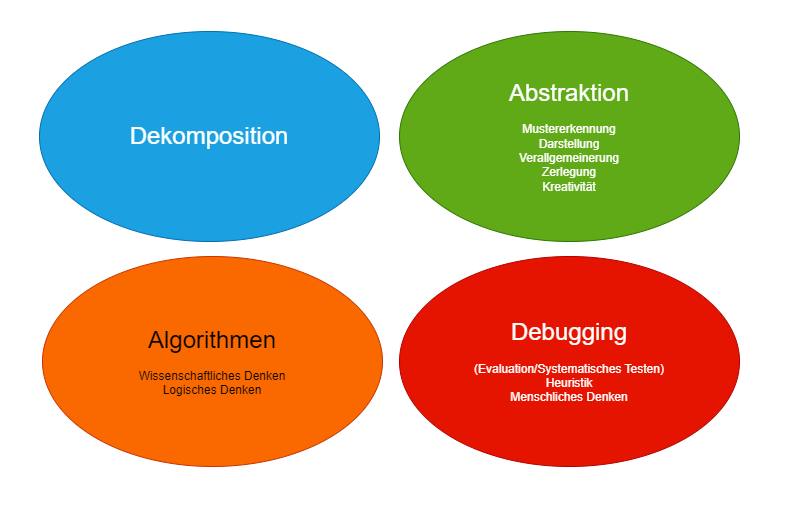
\includegraphics[width=1\linewidth]{Figures/Section_2/CT}
    \caption{Die Haupt- und Unterkategorien Computational Thinking aus verschiedenen Forschungen, grafisch dargestellt}
\end{figure}

Die Arbeit konzentriert sich auf die vier CT Aspekte, die im ersten Abschnitt definiert wurden.

\subsection{Lerntypen}
Um genau zu definieren, welchen Studierenden FP helfen kann, müssen zunächst konkrete Kategorien für die Typen von Lernenden festgelegt werden. Um zu analysieren, welche Studierenden möglicherweise Vorteile beim Erlernen von Programmierung haben könnten, werden diese Kategorien von Lerntypen im Zusammenhang mit CT und den jeweiligen Paradigmen betrachtet.

Ebenso wie im Feld des CT gibt es für Lerntypen kein allgemein akzeptiertes Modell. Allerdings gibt es einige Theorien, die häufiger, besonders im Kontext der Informatik, angewandt werden. Ein verbreitetes Modell ist hierbei das Felder-Silverman Lerntypenmodell (FSLSM) \cite{felder}. 
Das FSLSM wurde speziell im Kontext hoher Abbruchraten in Studiengängen der Ingenieurwissenschaften untersucht, wird allerdings auch vermehrt als Grundlage für Studien im Feld der Informatik verwendet \cite{kumar}.
Um die Lerntypen in der Forschungsgrundlage zu definieren, wird sich an diesem Lerntypenmodell orientiert.

\subsubsection{Differenzierung im Vergleich zu anderen Modellen}
Das FSLSM versteht sich nicht als völlig neues oder umfassendes Modell, und basiert auf bereits existierenden Modellen von etwa Jung \cite{jung}, Kolb \cite{kolb} und Briggs \cite{myers}.
Zudem sind die Lerntypen nicht so eindeutig bestimmbar, wie es herkömmliche Modelle, zum Beispiel das weit verbreitete VARK Modell von N. Fleming suggerieren.
Beispielsweise nutzen alle Menschen sowohl fühlende als auch intuitive Fähigkeiten, bevorzugen allerdings tendenziell eine der beiden Methoden. Das Lernmodell basiert nicht auf festen physischen Merkmalen, sondern auf differenzierteren Präferenzen der Subjekte, und betont, dass schwächere Lerntypendimensionen erlernt werden können.

Das FSLSM beschreibt vier verschiedene Bereiche, in denen sich die Lernstile größtenteils unterscheiden \footnote{Ursprünglich als 5 Bereiche definiert, wobei die Dimension "Inductive Deductive" nachträglich aus dem Modell entfernt wurde. Als Grund hierfür wurde angegeben, dass die meisten Schüler und Studierende einen schlussfolgernden Stil zwar präferieren, aber induktive Methoden in den meisten Fällen laut der Ansicht der Autoren objektiv besser für das Verständnis der Lernenden sind \cite{felder}.}. Hierbei wird immer jeweils ein Gegensatzpaar beschrieben, in das sich Subjekte einsortieren lassen. Die meisten Personen präferieren demnach einen der beiden Stile jeder Kategorie.

% Kurze Zusammenfassung der Lerntypen
\begin{description}
    \item[Sensorisch und Intuitiv] Dieser Aspekt beschäftigt sich damit, wie Personen am besten die Welt um sich herum wahrnehmen können. Hierbei präferieren Personen gewöhnlich eine der beiden Methoden, auch wenn alle Menschen beide verwenden können. Sensorische Typen präferieren, Daten und Fakten auswendig zu lernen, und sich länger mit den Details eines Problems zu beschäftigen. Sie ziehen es vor, einen klar erkennbaren Bezug auf die echte Welt zu haben und Probleme mit etablierten Methoden zu lösen. Intuitive Typen hingegen können ihre Umgebung besser durch eigene Theorien, Vorstellungen und Vermutungen wahrnehmen und setzen auf Innovation und Unsicherheiten. Sie sind besser darin, Abstraktion anzuwenden, und lernen neue Konzepte normalerweise schneller als sensorisch veranlagte Personen.
    \item[Visuell und Verbal] Dieser Aspekt beschäftigt sich mit der Art, wie Personen Input verarbeiten und Informationen am besten verstehen können. Visuelle Typen lernen am besten damit, was sie sehen können, etwa Diagramme, Bilder, Filme und Demonstrationen. Verbale Typen ziehen mehr aus Worten, sowohl geschriebenen als auch gesprochenen Erklärungen. Ihnen können besonders Gruppenarbeiten dabei helfen, das Material zu verstehen. Die Mehrheit der Lernenden hat typischerweise eine stärkere Ausprägung des visuellen Lerntypen, was im Konflikt mit den typischen Stilen von Vorlesungen in den Bereichen Informatik und Ingenieurswissenschaften steht. Hierbei wird meist ein frontaler Input gegeben, der im Großteil auf verbalen Vermittlungen basiert.
    \item[Aktiv und Reflexiv]  Dieser Aspekt beschäftigt sich mit der Verarbeitung von Informationen zum Wissen. Aktive Typen sind demnach besser darin, ihr Wissen direkt in der Anwendung zu vertiefen. Sie präferieren Gruppenarbeiten, in denen sie sich aktiv einbringen können, und lernen mit herkömmlichen Vorlesungsstilen nicht so effektiv. Reflexive Typen hingegen benötigen Zeit, um sich eigenständig mit Inhalten auseinanderzusetzen. Sie ziehen es vor, alleine zu arbeiten, und zuerst alle Fakten durchzudenken, bevor sie ein Problem angehen können.
    \item[Sequenziell und Global] Dieser Aspekt beschäftigt sich mit damit, wie Lernende Zusammenhänge verstehen. Sequenzielle Typen können besser in einer festgelegten logischen Reihenfolge arbeiten, etwa chronologisch, mit einem Buch oder mit den Inhalten einer Vorlesung. Globale Typen hingegen lernen oft sprunghaft und nicht linear, und müssen zunächst eine große Menge an Informationen ansammeln, bevor sich für sie das Gesamtbild erschließt. Da viele herkömmliche Vorlesungsformen auf einer schrittweisen Einführung der Konzepte basieren, haben globale Typen beim Erlernen neuer Sachinhalte normalerweise einen Nachteil gegenüber sequenziellen Lerntypen.
\end{description}

% SEC 3
\clearpage
\section{Forschungsteil}
\label{sec:work}

Um die Frage zu beantworten, ob es bestimmte Hänge zu einem oder dem anderen Paradigma gibt, muss zuerst beantwortet werden, wie die Paradigmen mit den Lerntypen zusammenhängen. 
Dazu wird untersucht, welche Lerntypen Vorteile beim Lernen der Computational Thinking (CT) Aspekte haben könnten. Außerdem wird geprüft, welche Empfehlungen Felder und Silvermann für die Lerntypen geben und wie diese mit den Eigenschaften der Paradigmen zusammenhängen.
Hierbei wird Objektorientierung (OO) mit FP verglichen. OO wurde hier als Vergleichspunkt gewählt, da es das häufigste Paradigma in Einführungskursen der Informatik ist. FP wird betrachtet, da es den Fokuspunkt der Arbeit darstellt. Andere Programmierparadigmen werden zunächst ausgelassen.
Abschließend wird untersucht, welche Rolle die CT Aspekte in den unterschiedlichen Paradigmen spielen, um zu bestimmen, ob ein Paradigma besondere Vor- und Nachteile aufweist.

% Disclaimer
Es werden hierbei vermehrt Annahmen zu den Vorlieben der Lerntypen gemacht, aufgrund der Empfehlungen von Felder und Silvermann in Relation zu den Merkmalen der Paradigmen. Aufgrund der zeitlichen Beschränkung der Arbeit können diese Annahmen nicht empirisch überprüft werden.

\subsection{Lerntypen im Zusammenhang mit Computational Thinking}
Das Erlernen von Programmierkenntnissen umfasst nicht nur das Schreiben von Code, sondern auch den Erwerb von CT Kompetenzen.
Nicht jede Lerntypendimension zeigt Vor- oder Nachteile beim Lernen der CT Aspekte, allerdings lassen sich einige klare Zusammenhänge herausstellen.

\subsubsection{Verbal Visuell}
Visuelle Lerner können einen Vorteil beim Erlernen von Abstraktion haben, da grafische Darstellungen eine sehr geeignete und beliebte Form ist, um das Konzept von Abstraktion zu erklären. Beispielsweise in der Objektorientierung werden hierbei öfters Bilder von Objekten wie Tieren oder Fahrzeugen verwendet, die dann auf Codeblöcke abstrahiert werden.
In der Informatik werden oft Vorlesungen mit starkem verbalen Input gehalten, was für verbale Lerntypen einen Vorteil bieten kann.
Zudem können visuelle Lerntypen bei der Dekomposition möglicherweise einen Vorteil, je nach Vorlesungsform haben. Ein Vorteil wäre hier möglich, wenn beispielsweise für das Aufteilen der Verantwortungen eines Klasse in der OO Programmierung grafische Darstellungen genutzt werden.

\subsubsection{Reflektiv Aktiv}
Reflektive Lerner könnten einen klaren Vorteil im Aspekt Debugging haben. Sie sind eher dazu veranlagt, ihre gefundenen Lösungen zu evaluieren und zu hinterfragen. Es ist demnach wahrscheinlicher, dass ein reflektiver Lerner von Natur aus Konzepte des Debugging anwendet. Aktive Lerner hingegen sind risikobereiter und sind in ihrer Arbeit experimentierfreudiger. Ihr Ansatz ist es eher, schnell zu scheitern, aber auch schneller neue Lösungen auszuprobieren.

\subsubsection{Sensorisch Intuitiv}
Intuitive Lerner haben einen klaren Vorteil in der Abstraktion \cite{felderhandout}. Dies ist der Fall unter anderem, da sie sich eher mit Konzepten statt Auswendiglernen beschäftigen. Sie haben oft Schwierigkeiten in Kursen, die stark auf Formelanwendung und Wiederholung setzen, und bevorzugen stattdessen neue Theorien und Interpretationen.
Auch im algorithmischen Denken werden Personen mit einem Hang zu intuitivem Lernen einen Vorteil haben, da sie normalerweise Konzepte schneller lernen als sensorische Lerner. Sie ziehen Innovation den etablierten Methoden vor und meiden eher Repetition. Dies könnte im Aspekt des algorithmischen Denkens von Vorteil sein, um neue Ansätze für Probleme zu entwickeln. Besonders im Zusammenhang mit dem Aspekt des Debugging könnte diese Innovation zu schnelleren und effizienteren Lösungen führen.

\subsubsection{Sequentiell Global}
In dieser Lerndimension lässt sich ein Vorteil für sequentielle Lerntypen im Aspekt der Dekomposition erkennen. Das Herunterbrechen auf Teilprobleme ist nicht nur ein wichtiger CT Aspekt, sondern auch eine Veranlagung des sequentiellen Lerntypen, der es vorzieht, Probleme in einem "Step by Step" Ansatz anzugehen. Sie beschäftigen sich mit allen Teilproblemen, bevor sie die komplette Lösung entwickeln können. Sequentielle Lerner können die einzelnen Teile eines Problems angehen, ohne das große Ganze zu kennen. Sie haben daher einen entscheidenden Vorteil im Herunterbrechen der Teilprobleme im Vergleich zu globalen Lerntypen.

\subsection{Eignung der Lerntypen für die Programmierparadigmen}
Nachdem die Zusammenhänge zwischen den Lerntypen und CT Aspekten untersucht wurden, muss noch betrachtet werden, inwiefern sich die verschiedenen Lerntypen für die Programmierparadigmen eignen.
Auch bei den Lerntypen des Felder Silvermann Modelles lassen sich teilweise Hänge erkennen.

\subsubsection{Verbal Visuell}
Hinsichtlich der Unterscheidung zwischen visuellen und verbalen Typen lässt sich beidseitig argumentieren. Beim Erlernen von objektorientierten Konzepten wie Vererbung bieten sich visuelle Darstellungen wie Graphen an, ähnlich wie im Aspekt der CT Abstraktion.
Allerdings können visuelle Typen einfacher mathematische Konzepte und Formeln auf die Philosophien der funktionalen Programmierung übertragen und die Zusammenhänge besser verstehen. Da FP einen starken Zusammenhang mit der Mathematik hat, können durch gewohnte Strukturen von Formeln und Funktionen einfachere Parallelen gezogen werden.
Welcher Lerntyp hier einen besseren Vorteil hat, kommt allerdings sehr auf die Strukturierung der Vorlesung an.

\subsubsection{Reflektiv Aktiv}
In der aktiven und reflektiven Dimension lässt sich in beiden betrachteten Paradigmen ein Vorteil für den reflektiven Typen erkennen. Die praktische Umsetzung von Programmierkenntnissen erfolgt meistens in Einzelarbeit und erfordert eine stetige Reflexion des Lerners.
Das Erlernen von Programmierkenntnissen könnte zwar auch in Gruppenarbeiten erfolgen, aber der typische Vorlesungsstil begünstigt eher den reflektiven Lerntypen.

\subsubsection{Sensorisch Intuitiv}
In dieser Dimension lassen sich klare Präferenzen für bestimmte Paradigmen erkennen. Sensorische Typen werden höchstwahrscheinlich OO bevorzugen. Die Klassen der OO modellieren Objekte der echten Welt und haben somit einen einfach verständlichen Bezug auf echte Probleme.
Intuitive Typen hingegen sind besser darin, Abstraktion anzuwenden, und werden daher eher FP bevorzugen.
Ihr Hang zu Innvoation und abstrakteren Konzepten ohne direkten Bezug zur realen Welt bietet ihnen einen Vorteil im Verständnis und in der Umsetzung von FP.

\subsubsection{Sequentiell Global}
Auch in der sequentiell globalen Dimension lassen sich klare Zusammenhänge zu den Paradigmen erkennen. Globale Lerntypen werden es höchstwahrscheinlich vorziehen, zunächst eine OO Klasse als Ganzes zu betrachten, bevor sie sich mit der Implementierung von Details beschäftigen. Um eine sinnvolle Hierarchie zur Komposition der verschiedenen Klassen zu entwerfen, muss grundlegend ein globaleres Verständnis der Probleme vorhanden sein.
Sequentielle Typen hingegen werden eher FP bevorzugen, da das Paradigma das Herunterbrechen von Problemen in Teilschritte von Grund auf vorsieht. Die Probleme werden in Teilfunktionen behandelt, und erst zum Schluss ergibt sich der Zusammenhang zu einem Programm. Ein globales Verständnis der Lösung ist nicht von Anfang an erforderlich.

\subsection{Ausprägung der Computational Thinking Aspekte in den Programmierparadigmen}
Um die Zusammenhänge zwischen den Vor- und Nachteilen herzustellen, muss betrachtet werden, wie genau die einzelnen CT Aspekte in den Paradigmen ausgeprägt sind. Kein Aspekt kann in einem Paradigma vollständig ausgelassen werden, da CT generell für das Konzept des Programmierens benötigt wird. Allerdings beeinflussen die unterschiedlichen Schwerpunkte und Philosophien der Paradigmen, wie die Aspekte gewertet und gewichtet werden können.
Aufgrund dieser Analyse können dann zusätzliche Schlüsse und Wichtungen der Vor- und Nachteile der Lerntypen gezogen werden.
% Hierzu wurde keine Forschung gefunden, deswegen sind das alles eigene Schlüsse (Fazitmaterial)

\subsubsection{Dekomposition}
In der FP ist die Dekomposition sehr stark ausgeprägt. Jede Funktion hat nur eine einzige Verantwortung und gibt immer dasselbe Ergebnis wieder. Durch Vermeidung von Seiteneffekten ist die Funktionsweise jeder Methode eindeutig. Der Programmablauf ist eher eine Abfolge von Befehlen als in der OO. In der OO erfolgt die Dekomposition nicht gezwungenermaßen auf Funktionsebene, sondern eher durch die einzelnen Klassen und deren Verantwortung.
\\
Da in der FP die Dekomposition einen starken Fokus hat, könnten hierbei visuelle Lerntypen eventuell einen zusätzlichen Vorteil hinsichtlich des funktionalen Paradigmas mit sich bringen, je nachdem wie die Dekomposition in der Vorlesung behandelt wird.

\subsubsection{Abstraktion}
Die Abstraktion in OO ist generell einfach zu visualisieren. Meistens werden die Probleme auf Klassen mit jeweils eigenen Funktionen heruntergebrochen. Diese Klassen wiederum können in Diagrammen oder Bildern mit ihren Funktionen dargestellt werden.
In der FP ist die Abstraktion stark mit der Dekomposition verknüpft. Um die einzelnen Teilfunktionen zu entwerfen, muss das Problem zunächst in die kleineren Einheiten zerlegt werden.
Es gibt eine sehr starke Abstraktion bis hin zu mathematischen Funktionen.
\\
Da intuitive Typen tendenziell einen Vorteil in Abstraktion haben, könnten ihnen das Erlernen von FP insgesamt leichter fallen.

\subsubsection{Algorithmen}
OO Sprachen bieten häufig ein breites Toolset für die Algorithmenentwicklung. Beispielsweise in Java sind Integer eine eigene Klasse, mit jeweils eigenen Operationen, die bei der Entwicklung verwendet werden können. In der FP hingegen ist das Toolset deutlich begrenzter, auch durch die Abwesenheit von Zuständen.
\\
Da FP stark auf innovative Lösungsansätze setzt, können intuitive Lerner hier besonders profitieren.
Außerdem könnten sequentielle Lerntypen einen zusätzlichen Vorteil in der FP haben. Die Umsetzung der Teilprobleme erfolgt isoliert voneinander und wird erst zum Schluss wieder in der Funktionskomposition zusammengesetzt. Ein globales Verständnis des Problems ist daher weniger essenziell als in der OO Programmierung.

\subsubsection{Debugging}
In der OO gibt es häufiger ein "klassisches" Debuggen. Klassen können diesen Prozess möglicherweise unübersichtlicher machen als in der FP. FP hingegen setzt stark auf Fehlervermeidung, indem Funktionen keine Seiteneffekte haben und deterministisch sind. Durch die eindeutige Verantwortung jeder Funktion treten weniger Flüchtigkeitsfehler oder unbeabsichtigte Nebeneffekte auf. Statt klassischem Debugging müssen Entwickler ständig reflektieren, und Fehler in der Funktionskomposition und in der Datenflusslogik finden.
Code in funktionalen Programmiersprachen benötigt daher generell weniger nachträgliche Bugfixes.

\begin{figure}[H]
    \centering
    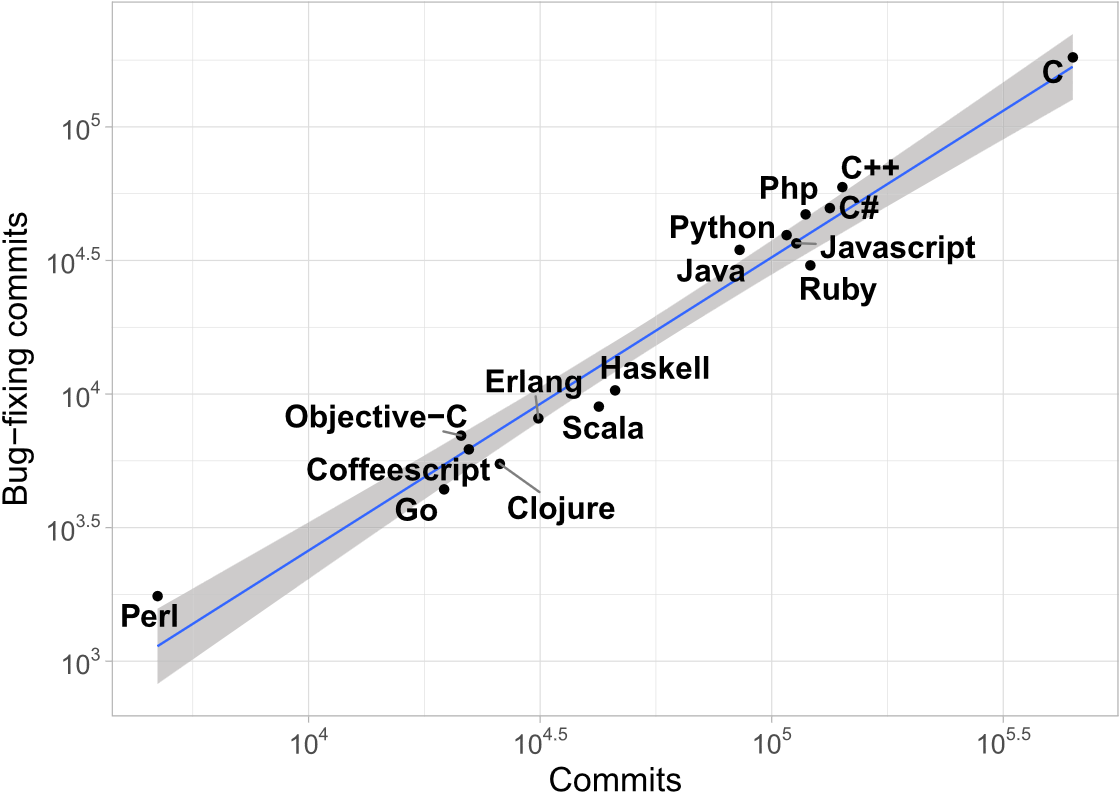
\includegraphics[width=1\linewidth]{Figures/Section_3/FigBugCommitsFP}
    \caption{Commits und Bugfixing Commits in verschiedenen Programmiersprachen \protect\cite{berger}}
\end{figure}

Aufgrund der besonders ausgeprägten Anforderung an die Reflexion beim Schreiben des Codes haben reflektive Typen möglicherweise einen zusätzlichen Vorteil in der FP.
Debugging in der FP erfordert ein abstraktes Verständnis der Vorgänge und eine ständige Reflexion der Arbeitsschritte.

\subsection{Zusammenfassung}
Zusammengefasst lassen sich also definitiv Hänge der Lerntypen zu bestimmten Paradigmen erkennen. In diesem Abschnitt werden die Vor- und Nachteile besonders im Hinblick auf die FP noch einmal übersichtlich dargestellt.

\begin{figure}[H]
    \centering
    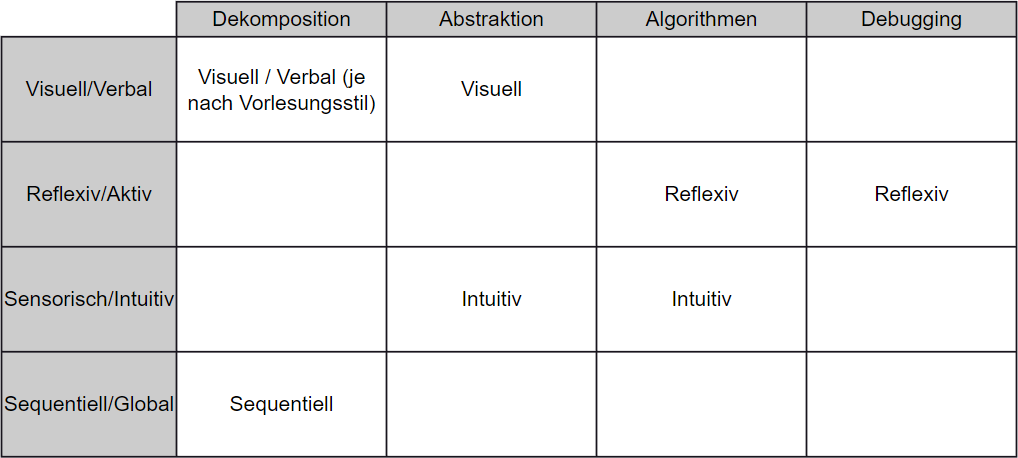
\includegraphics[width=1\linewidth]{Figures/Section_3/Styles_CT}
    \caption{Vorteile der Lerntypen in den Aspekten des Computational Thinking}
\end{figure}

Für die CT Aspekte lässt sich zusammenfassend sagen, dass besonders Personen mit visuell, reflektiv, intuitiv und sequentiell ausgeprägten Veranlagungen einen Vorteil beim Erlernen der einzelnen Aspekte haben.

\begin{figure}[H]
    \centering
    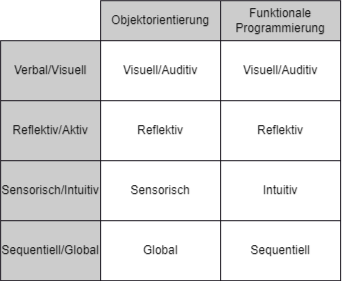
\includegraphics[width=1\linewidth]{Figures/Section_3/Styles_Paradigms}
    \caption{Vorteile der Lerntypen in den betrachteten Paradigmen}
\end{figure}

Für die Lerntypen lässt sich zusammenfassend sagen, dass besonders Personen mit reflektiv, intuitiv und sequentiell ausgeprägten Veranlagungen Vorteile beim Lernen mit funktionaler Programmierung haben.
Personen mit reflektiv, sensorischen und global ausgeprägten Eigenschaften hingegen werden besser mit OO Programmierung lernen.
Je nach Vorlesungsinhalt könnte ein visuell ausgeprägter Lerntyp noch einen zusätzlichen Vorteil in beiden Paradigmen haben.

\begin{figure}[H]
    \centering
    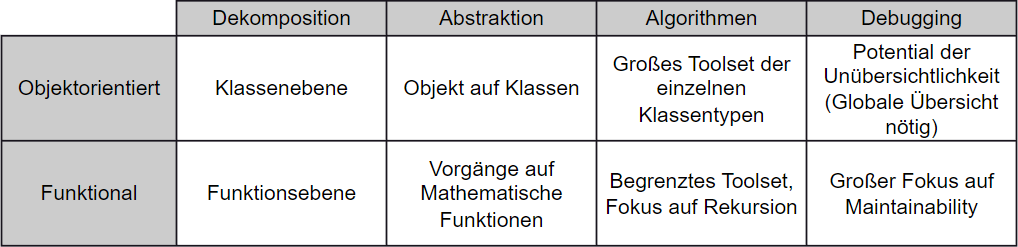
\includegraphics[width=1\linewidth]{Figures/Section_3/CT_Paradigms}
    \caption{Ausprägungen der CT Aspekte in den jeweiligen Programmierparadigmen}
\end{figure}

Zu den einzelnen Ausprägungen der CT Aspekte in den Paradigmen lassen sich zusätzliche Vorteile der Lerntypen ziehen.
Hat ein Lerntyp beispielsweise sowohl einen Vorteil beim Erlernen von algorithmischem Denken, als auch eine Neigung zu innovativen Lösungsansätzen, etwa durch eine besondere Ausprägung der intuitiven Lerntypendimension, wird dieser sich auch mit dem Toolset der FP leichter tun.

\subsubsection{Vorteile der Lerntypen in funktionaler Programmierung}
Durch die Analyse sowohl der Programmierparadigmen als auch der Computational Thinking Aspekte hinsichtlich der Lerntypen haben sich klare Vorteile einiger Ausprägungen ergeben.
Insbesondere folgende Lerntypen werden demnach Vorteile haben, wenn sie ihren Programmiereinstieg mit funktionaler Programmierung machen.

\begin{description}
    \item[Visuell] Da ein direkter Bezug zu mathematischen Formeln gemacht werden kann. Zudem haben visuelle Typen einen Vorteil in der Dekomposition.
    \item[Reflektiv] Da Programmierung tendenziell eher in Einzelarbeit erfolgt, und der Lerntyp in herkömmlichen Vorlesungsstilen besser unterstützt wird. Zudem profitiert der reflektive Typ stark durch die Fehlervermeidungsstrategie von FP. Durch ständige Reflexion der Teillösungen können potenzielle Fehler früh erkannt werden.
    \item[Intuitiv] Da dieser Typ in der FP einen besonderen Vorteil in der Abstraktion hat, die in der FP essenziell ist, da die meisten funktionalen Programmiersprachen auf dem Lambda-Kalkül basieren. Da Innovation bei neuen Algorithmen wichtig in der FP ist, hat dieser Typ auch hier einen Vorteil.
    \item[Sequentiell] Da FP einen eher sequentiell veranlagten Entwicklungsstil hat, in dem ein Teilproblem nach dem anderen angegangen wird. Zudem kann eine sequentielle Veranlagung zusätzlich bei der Erlernung von Dekomposition helfen.
\end{description}

Diese Ausprägungen decken sich zudem mit den ausgearbeiteten Vorteilen zum Erlernen von CT Aspekten, was einen zusätzlichen Vorteil bieten kann.
\\
\subsubsection{Nachteile der Lerntypen in funktionaler Programmierung}

Andererseits haben im Umkehrschluss zum vorherigen Abschnitt wiederum folgende Lerntypen eher Nachteile bei FP.

\begin{description}
    \item[Verbal] Da verbal schwieriger ein Bezug zu den mathematischen Grundlagen von FP gemacht werden kann.
    \item[Aktiv] Da die Programmierung allgemein reflektive Typen bevorzugt. Zudem widerspricht ein aktiver Stil der Fehlervermeidung in FP, da diese eine ausführliche Reflexion der Arbeitsschritte erfordert.
    \item[Sensorisch] Da nicht so ein guter Bezug zu echten Problemen hergestellt werden kann. Zudem hat ein sensorischer Typ eher Nachteile beim Erlernen von Abstraktion und beim innovativen Ausarbeiten von neuen Lösungen für Probleme. Das Anwenden etablierter Methoden ist besonders beim Erlernen von FP schwieriger, da sich das Paradigma von anderen Programmierstilen stark unterscheidet.
    \item[Global] Da eher ein sequentielles Denken gefordert ist. In der OO ist ein globales Denken von Vorteil, da der Zusammenhang zwischen den Domänen eine Rolle spielt und ein Verständnis der gesamten Architektur nötig ist. In der FP allerdings werden die Probleme eher schrittweise angegangen, was für diesen Lerntypen ein Nachteil sein könnte.
\end{description}
% SEC 4
\clearpage
\section{Praxis}
\label{sec:practice}

Kurze Einleitung in den Sinn und Hintergrund des Praxisteiles

\subsection{Lerntypenanalyse}
Um das Selbstexperiment in Verbindung mit den Vor- und Nachteilen der Lerntypen in den verschiedenen Feldern setzen zu können, musste zunächst eine eigene Lerntypen Analyse durchgeführt werden.
Hierzu wurde der "Index of Learning Styles Questionnaire" Fragebogen verwendet \cite{ils_questionnaire}, ein Online Tool welches insgesamt 44 Fragen stellt, und dann auf Basis der Antworten sowohl die Lerntypen eines Individuums einschätzen kann. Die Lerntypen, die als Gegensatzpaare definiert sind, befinden sich auf einer 2 Dimensionalen Skala, die einschätzen soll, wie ausgeprägt der Hang zu einem Aspekt ist. Verwendet wurde hierbei die PDF Version des Fragebogens. Ein Wert von 1 bis 3 entspricht einer ausgewogenen Balance beider Aspekte der Dimension. Ein Wert von 5 bis 7 entspricht einem mäßigem Hand zu einem Aspekt. Ein Wert von 9 bis 11 entspricht einer starken Präferenz eines Lernstiles in der Dimension.
Die Verlässlichkeit dieses Fragebogens wurde mehrmals, sowohl von den ursprünglichen Autoren des Lernmodelles \cite{felder2005}, als auch von anderen Quellen \cite{zywno}, geprüft und bestätigt.

\subsubsection{Ergebnisse der persönlichen Evaluierung}
Die Fragen des ILS Fragebogens wurden in einer zufälligen Reihenfolge beantwortet, um zu vermeiden, dass bereits vorab klar ist, welche Frage welcher Typendimension korrespondiert. Dies ist möglich, da der Test so aufgebaut ist, dass jeweils ein Frageblock von 4 Fragen jede Dimension behandelt. Die erste Frage beispielsweise geht in die Wertung der Aktiv/Reflektiven Dimension ein, die 5 Frage beschäftigt sich wieder mit der Dimension, und die 9 Frage ebenfalls.

Die Fragen des ILS-Fragebogens wurden in zufälliger Reihenfolge beantwortet, um zu verhindern, dass bereits im Voraus offensichtlich ist, welche Frage welcher Dimension zugeordnet ist.
Dies ist möglich, da der Test so konzipiert ist, dass jede Dimension in Blöcken von vier Fragen abgedeckt wird. Beispielsweise fließt die erste Frage in die Bewertung der Aktiv/Reflexiv-Dimension ein, die fünfte Frage ebenfalls und ebenso die neunte.

Die Ergebnisse des Fragebogens lauten wie folgt.

\begin{figure}[H]
    \centering
    \newcolumntype{C}{>{\centering\arraybackslash}X}
\begin{tabularx}{\textwidth}{l C C C C C C C C C C C C l}
    ACT & 11a & 9a & 7a & 5a & 3a & 1a & 1b & \colorbox{BurntOrange}{\textbf{3b}} & 5b & 7b & 9b & 11b & REF \\
    SEN & 11a & \colorbox{BurntOrange}{\textbf{9a}} & 7a & 5a & 3a & 1a & 1b & 3b & 5b & 7b & 9b & 11b & INT \\
    VIS & 11a & 9a & \colorbox{BurntOrange}{\textbf{7a}} & 5a & 3a & 1a & 1b & 3b & 5b & 7b & 9b & 11b & VRB \\
    SEQ & 11a & 9a & 7a & 5a & 3a & 1a & \colorbox{BurntOrange}{\textbf{1b}} & 3b & 5b & 7b & 9b & 11b & GLO \\
\end{tabularx}
    \caption{Ergebnisse des ILS Fragebogens, visualisiert}
\end{figure}

Demnach lässt sich schließen dass der Autor Hänge zu folgenden Dimensionen aufweist.

\begin{itemize}
    \item Ein ausgewogenes Verhältnis der Aktiven/Reflektiven Dimension
    \item Ein starker Hang zum sensorischem Typen 
    \item Ein mäßiger Hang zum visuellen Typen
    \item Ein ausgewogenes Verhältnis der Sequentiellen/Globalen Dimension
\end{itemize}

% Problem as I am writing this ist Section 3 noch nicht so ganz fertig und das hier könnte daher noch anders ausfallen

Die Hänge der einzelnen Lerntypen wird im praktischen Versuch anschließend in Bezugzu den Vor- und Nachteilen für das Erlernen und Anwenden der Computational Thinking Aspekte und der verschiedenen Paradigmen gesetzt.
Theoretisch sollte es in folgenden Bereichen Vor- und Nachteile geben.

\begin{itemize}
    \item Ein Vorteil beim Anwenden von Abstraktion
    \item Ein Vorteil im Aspekt des Debuggens, und der Analyse der gefundenen Lösungen
    \item Ein möglicher Nachteil beim algorithmischen Denken insgesamt
    \item Kein klarer Vor- oder Nachteil in der Dekomposition, aufgrund eines ausgewogenen Verhältnisses in der sequentiell/globalen Dimension
\end{itemize}

\subsection{Problembeschreibung}
% SEC 5
\clearpage
\section{Fazit}
\label{sec:conclusion}

Abschließend werden noch einmal alle Ergebnisse der Bachelorarbeit insgesamt betrachtet und in Beziehung zueinander gesetzt. Zudem erfolgt eine kurze Reflexion zum Prozess der Arbeit, sowie mögliche Erweiterungen der Forschungsfrage in zukünftigen Arbeiten.

\subsection{Schlussfolgerungen aus Theorie und Praxis}
Abschließend lässt sich also sagen, dass die Ergebnisse der Arbeit darauf hindeuten, dass ein Zusammenhang zwischen den verschiedenen Lerntypen und ihrer Eignung für funktionale Programmierung (FP) besteht.
Im Verlaufe der Arbeit wurden sowohl Vor- als auch Nachteile für die einzelnen Lerntypendimensionen identifiziert und mithilfe eines Selbstversuches analysiert. Die Erkenntnisse legen nahe, dass Probleme von Programmieranfängern möglicherweise reduziert werden können, wenn die Stärken und Schwächen dieser berücksichtigt werden. Dies könnte zu einer geringeren Abbruchrate beitragen, und den Einstieg in das Studium für neue Studierende generell einfacher gestalten.

Im Hinblick auf die zu Beginn formulierten Forschungsfragen lassen sich folgende Schlussfolgerungen ziehen.

\begin{enumerate}
    \item \textbf{Fällt es jedem gleich leicht, Programmieren zu lernen, oder gibt es Hänge zu einem bestimmten Paradigma?} Abschließend lässt sich sagen, dass Hänge zu Paradigmen erkannt wurden. Welche Paradigmen von wem bevorzugt werden, hängt von den individuellen Lerntyp-Präferenzen ab, könnte allerdings auch von der Gestaltung der Vorlesungen beeinflusst werden.
    \item \textbf{Welche Vor- und Nachteile haben gängige Paradigmen für die jeweiligen Lerntypen?} Es wurden im Laufe der Arbeit eindeutige Vor- und Nachteile für FP und objektorientierte (OO) Programmierung gefunden. Andere Paradigmen wurden zunächst nicht betrachtet, könnten allerdings in der Zukunft auch in den Kreis der zu betrachtenden Paradigmen aufgenommen werden.
    \item \textbf{Welchen Lerntypen würde funktionale Programmierung beim Lernen von Entwicklung helfen, und welchen Typen würde der Ansatz eher schaden?} Im Forschungsteil der Arbeit konnte eindeutig identifiziert werden, welche Kombination von Ausprägungen der Lerntypdimensionen ein Lernen von FP besonders begünstigt.
\end{enumerate}

\subsection{Reflexion}
Dieser Abschnitt betrachtet die Umsetzung der Bachelorarbeit in Hinsicht auf die ursprünglich geplante Durchführung und wägt ab, wieso Schwierigkeiten auftraten, und welche Verbesserungen sinnvoll wären.

\subsubsection{Erfolge}
Einige Aspekte der Bachelorarbeit fielen leichter als zunächst angenommen. Besonders hat hierbei das Felder-Silverman Lerntyp Modell (FSLSM) geholfen. Dies konnte man sehr gut in den Kontext der Informatik setzen, unter anderem weil das Modell auch in der Vergangenheit in anderen Studien des Feldes als Richtlinie verwendet wurde.

Die Autorinnen des Modells legen zudem einen besonderen Wert darauf, dass das Modell und die Theorie weiterhin frei zugänglich bleiben, und stellen auf ihrer Webseite sehr viele Links und Ressourcen zur Verfügung. Die Ressourcen beinhalten unter anderem auch Belege zur Verlässlichkeit des Lerntypenmodell-Fragebogens, was die Entscheidung zur Verwendung des Modells als Mittel sehr einfach machte.

Der Fragebogen der offiziellen Seite war zunächst nicht funktional, aber auf Anfrage stellte sich heraus, dass dies daran lag, dass international versucht wurde, auf eine Webseite der University of Pennsylvania zuzugreifen. Mithilfe eines Virtual Private Networks (VPN) konnten diese Probleme behoben werden, und die Seite konnte normal verwendet werden.

Weiterhin war das Lernen mithilfe des Kurses der University of Pennsylvania sehr hilfreich. Der Kursinhalt war leicht verständlich und gut aufgebaut. Als Vorbereitung auf den praktischen Selbstversuch wurden einige Übungsaufgaben des Kurses bearbeitet. Dies half erheblich mit dem Erlernen der Haskell Syntax und der generellen Denkweise von FP.

\subsubsection{Schwierigkeiten}
Eines der frühesten Probleme der Bachelorarbeit fand sich im Rechercheteil. Zum Begriff Computational Thinking (CT) ließ sich keine einheitliche Definition finden, und es war sehr schwer abzuwägen, welche Studien am vertrauenswürdigsten sind.
Um diesem entgegenzuwirken, wurden mehrere Studien und Literatur zu dem Thema betrachtet, die es sich vornehmen, die bisherigen Forschungsergebnisse aller Studien zusammenzufassen und auf einen einheitlichen Stand zu bringen. Um eine möglichst objektive Auswahl zu treffen, wurden vier Aspekte gewählt, die in der Forschung am häufigsten diskutiert und untersucht wurden. Hierzu wurden mögliche Unteraspekte unter größeren CT Aspekten gruppiert.

Zudem war eines der größten Probleme der Bachelorarbeit, einen Zusammenhang der drei Themenfelder, CT, FP und das FSLSM, zu finden. Es wurde ein klarer Zusammenhang zwischen CT und den Lerntypen, sowie FP und den Lerntypen gefunden. Diese Vor- und Nachteile dann allerdings wiederum in der dritten Ebene zu kombinieren erwies sich als besonders zeitaufwendig.
Es war sehr schwierig zu bestimmen, wie CT und FP zusammenhängen, und welche Aspekte eine größere oder kleinere Rolle in den einzelnen Paradigmen spielen. Jeder CT ist in seiner eigenen Weise für das Programmieren allgemein wichtig.
Da es keine vorhandene Forschung zum Zusammenhang von Programmierparadigmen und CT gab, basieren die Ergebnisse dieses Abschnitts größtenteils auf eigenen Schlussfolgerungen und Annahmen.
Es wurden verschiedene Überschriften für die Themen entworfen, die die Gedankenprozesse ein wenig eingrenzten. Letztlich wurden die Abschnitte zunächst wieder gelöscht und durch eine stichpunktartige Herangehensweise neu formuliert, um die Gedanken klarer zu formulieren. Zudem half es, eine visuelle Zusammenfassung der Schlussfolgerungen der einzelnen Abschnitte in Form der Tabellenabbildungen zu haben. Auf die Visualisierungen wurde auch immer wieder zurückgegriffen.
Letztendlich orientierte sich die Struktur stärker an den Forschungsfragen als an der ursprünglich geplanten Gliederung der Abschnitte.

Eine weitere Schwierigkeit war insgesamt, die Forschungsfragen mit dem Selbstversuch zu belegen. Der Zweck des Selbstversuches war es, einen Programmieranfänger zu simulieren, der noch keine Erfahrungen in funktionaler Programmierung gemacht hat. Die Autorin hatte zwar keine funktionalen Programmierkenntnisse, allerdings bereits generelles Programmierwissen. Es bleibt daher unklar, inwiefern die bereits angeeigneten CT Aspekte in der Lösungsfindung geholfen haben. Insbesondere die Aspekte, in denen ein Vorteil gegeben war, also die Abstraktion und Dekomposition, sind Aspekte der Informatik, die im Verlaufe des Studiums immer wieder weitergebildet und trainiert werden.
Besonders bei der Implementierung fiel auf, dass eher auf herkömmliche prozedurale Denkstrukturen zurückgegriffen wurden, die anschließend in funktionale Funktionen umgewandelt wurden.
Stattdessen sollten die Programmierfähigkeiten von Grund auf mit funktionaler Programmierung betrachtet werden. Eine Diskussion dazu, wie dieses Problem umgangen werden könnte, findet sich im Abschnitt \nameref{sec:empirical}.

Zudem, als ein eher allgemeines Problem des Selbstversuches, war es sehr schwer und zeitaufwendig, sich mit der neuen Syntax von Haskell auseinanderzusetzen. Die Sprache ist fern genug von allen im Studium erlernten Programmierkenntnissen, um in der Bearbeitung eine Schwierigkeit darzustellen.
Das lokale Einrichten der Sprache, sowie die Verwendung der REPL war allerdings sehr einfach, und gab schnelles Feedback beim Durchführen der Aufgaben.

\subsection{Erweiterung der Forschungsfrage}\label{sec:future}
\subsubsection{Unterstützung von benachteiligten Lerntypen}
Ein Aspekt, der in der Arbeit vernachlässigt wurde, ist die Nachteilausgleichung. Laut des FSLSM sollen die Lerntypen idealerweise nicht als Richtlinie für Lernmethoden verwendet werden. Allerdings ist es möglich, Personen mit schwächer ausgebildeten Dimensionen der Lerntypen zu unterstützen.
Beispielsweise sind herkömmliche Vorlesungen in Informatikstudiengängen eher in einer Art und Weise strukturiert, die verbalen Lerntypen einen Vorteil bieten würden. Personen mit schwächer ausgebildeten verbalen Kompetenzen könnten dabei unterstützt werden, diese Kompetenzen zu entwickeln. Parallel könnte diesen Personen allerdings auch gefördert werden, erste CT Kompetenzen zu erwerben, damit diese über einen längeren Zeitraum nicht den Anschluss an die Lerninhalte verlieren. Im Feld der Informatik wäre dies zum Beispiel durch die Verwendung der blockbasierten, visuellen Programmiersprache Scratch möglich.
Letztendlich geht es nicht darum, allen Lerntypen gerecht zu werden, sondern gemeinsame Lösungen zu finden, die sicherstellen, dass alle im gleichen Tempo lernen können.

Die Frage, wie dieser gemeinsame Grund für alle Programmiereinsteiger in Studiengängen der Informatik mithilfe der Lerntypen gefunden werden kann, könnte eine eigene Forschungsfrage für eine zukünftige Arbeit sein. Hierbei könnten verschiedene Ansätze zur Umstrukturierung einer "klassischen" Vorlesung entwickelt werden und gegebenenfalls unter Studienanfängern der Informatik vorgestellt werden.

\subsubsection{Erweiterung der Curricula-Analyse}
Aufgrund des Zeitmangels und weil die Curricula-Analyse nicht der Schwerpunkt der Bachelorarbeit war, wurden die Daten ausschließlich auf verwendete Programmiersprachen sowie Paradigmen untersucht. Was allerdings noch eine interessante Erweiterung wäre, könnte sein, die Kursinhalte selbst noch näher zu untersuchen. Dazu könnten entweder die Modulhandbücher herangezogen werden, die allerdings begrenzte Informationen über die Vorlesungen selbst zur Verfügung stellen. Andererseits könnten ausgewählte Universitäten und Hochschulen kontaktiert werden, um Zugang zu den detaillierten Lehrinhalten zu erlangen.
Beispielsweise könnten die wenigen Kurse, die sich mit funktionaler Programmierung beschäftigen, darauf untersucht werden, wie tief die Lehrinhalte hier wirklich gehen. Wird beispielsweise FP in der Praxis angewandt? Oder wird diese nur in der Theorie gelehrt und ist möglicherweise nur Teil einer kurzen Übersicht über alle verbreiteten Programmierparadigmen?

\subsubsection{Untersuchung anderer Paradigmen in Hinsicht auf CT Aspekte und Lerntypen}
Im Rahmen der Bachelorarbeit wurde speziell OO und FP im Kontext CT und Lerntypen betrachtet. Bei der Curricula Analyse ist allerdings aufgefallen, dass oft OO und Prozedurale Programmierung zusammen gelehrt werden. Hierbei stellt sich die Frage, welche Kompetenzen die jeweiligen Ansätze besonders gut vermitteln können.
Möglicherweise gibt es noch ausgeprägtere Hänge der bestimmten Lerntypdimensionen zu einem anderen Paradigma, welches im Rahmen der Forschungsarbeit nicht betrachtet wurde.

\subsubsection{Untersuchung weiterer CT Aspekte}
Aufgrund dessen, dass es keine einheitliche Definition von CT gibt, wurden in der Arbeit die vier häufigsten Aspekte betrachtet. Es wurden allerdings zudem auch weitere Aspekte herausgestellt, die ebenso relevant für die Anwendung von CT sind. Diese Aspekte wurden im Rahmen der Arbeit nicht betrachtet, könnten allerdings in Zukunft ein weiterer Fokuspunkt einer weiterführenden Forschungsfrage sein. Hierbei könnten die zusätzlichen CT Aspekte weiter kategorisiert und hierarchisch geordnet werden.

\subsubsection{Untersuchung der Vor- und Nachteile in funktionaler Programmierung}\label{sec:empirical}
Aufgrund der zeitlichen Begrenzung wurde der praktische Versuch zur Untersuchung der Vor- und Nachteile der Lerntypen in funktionaler Programmierung mit der Autorin selbst durchgeführt. Da allerdings bereits vorher bekannt war, welche Lerntypen dieser besitzt, gab es einen gewissen Bias in der Untersuchung der Schwierigkeiten und Vorteile.
Um eine verlässlicherere Untersuchung durchzuführen, wäre es sinnvoll, den Versuch erneut anhand fremder Versuchspersonen durchzuführen, die sich im ersten Semester eines Informatikstudiums befinden.
Hierzu könnte ein sehr kurzer Einleitungskurs zu FP entworfen werden, anhand dessen die Probanden eine Aufgabe durchführen. Im Anschluss an den Programmierteil wird dann der Lerntyp der einzelnen Personen mittels des Felder Silverman Fragebogens festgestellt.

\subsubsection{Weitere Forschung zur Ausprägung der CT Aspekte in den Paradigmen}
Aufgrund dessen, dass im Rahmen der Bachelorarbeit wenige Quellen zum Thema CT im Zusammenhang mit Programmierparadigmen gefunden wurden, basieren die meisten Schlussfolgerungen des Forschungsteils auf eigenen Annahmen. Allerdings könnten die Ausprägungen der einzelnen CT Aspekte ebenfalls in der Praxis untersucht werden.
Durch die Stärken und Schwächen der einzelnen Lerntypen würden sich in einem praktischen Versuch möglicherweise Rückschlüsse darauf ziehen lassen, wie sich die Paradigmen auf einzelne CT Aspekte fokussieren.
Diese Art von Forschungsfrage könnte sich ebenfalls mit der Frage auseinandersetzen, wie man Programmieranfänger am besten in ihrem Lernprozess unterstützen kann.

% SEC 6
\clearpage
\section{Anhang}
\label{sec:appendix}

Im Anhang wird das Vorgehen in den verschiedenen Abschnitten näher erläutert. Es werden alle Hintergrundinformationen, die nicht direkt für die Arbeit selbst relevant sind, gesammelt und dargestellt.

\subsection{Vorgehen bei der Untersuchung der Curricula}
Um auszuarbeiten, wie die aktuelle Situation an deutschen Hochschulen und Universitäten ist, wurde der Hochschulkompass der Hochschulrektorenkonferenz verwendet \cite{hochschulkompass}.
Auf der Webseite wurden Studiengänge der Informatik gesucht und nach folgenden Kriterien mithilfe der Filterfunktion der Webseite sortiert:

\begin{itemize}
    \item Abschluss Bachelor/Bakkalaureus (Da Programmieranfänger betrachtet werden sollen, ergibt es im Kontext keinen Sinn, weiterführende Studiengänge oder Masterprogramme zu berücksichtigen)
    \item Studientyp Grundständig (Siehe Abschluss Bachelor/Bakkalaureus)
    \item Fachsuche Informatik (Speziellere Studiengänge wie Bioinformatik und Wirtschaftsinformatik wurden ausgeschlossen, um Überschneidungen zwischen den Hochschulen zu meiden. Es wurde immer ein Studiengang pro Institution untersucht, der sich möglichst nah an der Allgemeinen Informatik kategorisieren lässt)
    \item Studienfeld Angewandte Informatik oder Informatik (Siehe Fachsuche)
    \item Studienformen Vollzeitstudium (Ein weiteres Kriterium, um Überschneidungen zu meiden und die Studiengänge weiter auszusortieren)
    \item ohne Lehramt (Wurde in den Filtern aussortiert, da die Lerninhalte sowohl Informatik als auch Erziehungswissenschaften umfassen, und somit nicht im Fokus der Arbeit liegen)
\end{itemize}

Nach der Anwendung der Filter wurden noch insgesamt 425 Treffer angezeigt, die erst im späteren Verlauf der Arbeit weiter reduziert wurden (siehe \nameref{sec:sorting}).

\subsubsection{Zeit Verwaltung}\label{sec:time_management}
Da die Curricula-Analyse nicht der Schwerpunkt der Bachelorarbeit sein sollte, musste entschieden werden, wie viel Zeit in das Thema investiert werden soll.
Hierbei wurden mehrere Risiken gesehen. Zum einen ist es möglich, dass man durch Internetrecherche alleine nicht erschließen kann, welche Inhalte ein Modul hat.
Zum anderen ist das größere Risiko wahrscheinlich der Zeitfaktor. Es ist ungewiss, wie lange es dauert, jedes Modul zu untersuchen, da jede Institution ihre Informationen anders sortiert, bereitstellt und handhabt.

Um die Zeit in einem realistischen Rahmen zu halten, wurde in Erwägung gezogen, einen Zeitraum festzulegen, in dem so viele Studiengänge wie möglich betrachtet werden, und diese anschließend die Forschungsmenge darstellen. Dieser Zeitraum könnte etwa auf 2 Arbeitstage fallen. Auch wurde abgewägt, die Studiengänge nach Anzahl der Studierenden zu sortieren und die 50 am besten besuchten Institutionen zu betrachten.

Es wurde allerdings ebenfalls notiert, dass das unsicherste Kriterium hier die Zeit war, die benötigt wird, um einen Studiengang zu untersuchen. Möglicherweise müssen die Methoden zur Reduktion der Zeit gar nicht angewandt werden, wenn sich die Risiken nicht erfüllen. Zunächst wurde daher versucht, abzuwägen, wie lange Analysezeit grob einzuschätzen war.
In einer isolierten Probe wurden fünf zufällige Universitäten betrachtet (In diesem Fall die ersten fünf Suchergebnisse des Hochschulkompasses, die HS Furtwangen, die Ruhruniversität Bochum, die Hochschule Fulda, die Friedrich-Schiller-Universität Jena, und die Hochschule Konstanz).
Es dauerte etwa 10 Minuten, um entsprechende Informationen über alle 5 Studiengänge zu erlangen.
Bei den 121 verbleibenden Informatik-Studiengängen wurde die Zeitdauer also grob auf 4 Stunden eingeschätzt, ein realistischer Zeitraum zur Sammlung der Daten. Mit diesen neuen Informationen wurden die Methoden zur Zeitreduktion wieder verworfen.

Letztendlich wurde für die Analyse doch ein ganzer Arbeitstag benötigt, aber die reduzierte Menge der Studiengänge durch die Filter war bereits genügend, um die Daten in einem angemessenen Zeitraum zu sammeln.

\subsubsection{Untersuchung der Daten}\label{sec:sorting}
Bei der Analyse der Curricula wurde systematisch vorgegangen. Mithilfe eines Webscrapers wurden alle nötigen Informationen als JSON extrahiert und in einer Excel-Tabelle sortiert.
Es wurde festgestellt, dass die Filterfunktion des Hochschulkompasses nicht ausreichend war, um die Datenmenge zu reduzieren. Die Studiengänge wurden daher noch einmal manuell aussortiert, nach weiteren Kriterien.
Ein Studiengang wurde demnach aussortiert, wenn eines der folgenden Kriterien zutraf.

\begin{itemize}
    \item Kein allgemeiner Informatikstudiengang (Zum Beispiel Bioinformatik oder Wirtschaftsinformatik)
    \item Zweitfach oder Nebenfach Informatik
    \item Teilzeitstudium
    \item Mehrere Studienorte für einen Studiengang (Hierbei sind die angebotenen Module teils nicht eindeutig zuordenbar)
    \item Doppelte Studiengänge für eine Institution (Etwa wenn sowohl Angewandte als auch Allgemeine Informatik angeboten wird. Es wurde immer der allgemeinere Studiengang gewählt. Zwischen internationalen und deutschen Studiengängen wurde immer der deutsche Studiengang gewählt)
\end{itemize}

Für die meisten Studiengänge ließen sich die nötigen Informationen in sehr kurzen Zeiträumen mit einer Suche nach dem Studienverlaufsplan, sowie dem Modulhandbuch für die Informatik finden.
Hierbei wurde der Studienverlaufsplan genutzt, um herauszufinden, welcher Kurs als Einführung in die Programmierung im ersten Semester dient, und das Modulhandbuch, um zu extrahieren, welche Programmierparadigmen und Sprachen im Kurs verwendet werden.

\paragraph{Unterschied der Datensätze Unspezifisch und Keine Infos}\label{sec:unspecified_vs_na}
Nicht alle Module listeten die benötigten Informationen. Es wird in der Analyse grundsätzlich unterschieden zwischen zwei Fällen. Zum einen, Studiengänge, die zwar ein Modulhandbuch zur Verfügung stellten, dieses aber nicht explizit spezifiziert, welche Paradigmen und Programmiersprachen verwendet werden (Markiert als "Unspezifisch"). Zum anderen gibt es noch den Fall, dass kein Modulhandbuch öffentlich zur Verfügung steht. Dies kann etwa der Fall sein, wenn die Institution Informationen nur auf Anfrage herausgibt, oder das Modulhandbuch einfach nicht aufzufinden war. Es wurde davon abgesehen, die Institutionen zu kontaktieren, um einen neuen ungewissen Faktor in der Arbeit zu vermeiden. Die Studiengänge ohne Modulhandbuch wurden leer gelassen und sind in der Excel-Tabelle rot markiert. In der Grafik zur Darstellung der Ergebnisse sind diese Datensätze in "Keine Infos" kategorisiert.
\\
Die Excel-Tabelle mit den extrahierten Daten lässt sich im Repository der Bachelorarbeit finden \cite{repoxlsx}.

\subsection{Auswahl des Problems für den Selbstversuch}\label{sec:choice_prac}
Die Auswahl des Programmierproblems in Abschnitt 4 der Arbeit erfolgte an mehreren Kriterien. Es sollte ein relativ einfaches Problem gewählt werden, das eher einen Zweck demonstriert als kreative Lösungen erfordert.
Zunächst wurde hierbei entschieden, einen Algorithmus zur automatischen Lösung und Erstellung eines Sudoku zu schreiben.
Bei einem Sudoku handelt es sich um ein klassisches Rätsel, bei dem auf einem 9x9 großen Feld in jeder Zeile, Spalte, und in jeder 3x3 großen Box jede Zahl von 1 bis 9 nur ein mal vorkommen darf.

Das Problem eignete sich zum Untersuchen und Lernen von funktionaler Programmierung (FP), da alle wichtigsten Aspekte von FP benötigt wurden, um das Problem im Paradigma erfolgreich umzusetzen (Rekursion, Funktionen höherer Ordnung, Komposition, Unveränderlichkeit). Es wurden ebenfalls alle CT Aspekte ausreichend abgedeckt.

\begin{description}
    \item[Dekomposition] Herunterbrechen in Teilprobleme. Beispielsweise Validierung des Sudoku, dann Untersuchen der Spalten, Zeilen und Boxen separat.
    \item[Abstraktion] Rätsel in Datenstrukturen umwandeln. Beispielsweise Überlegungen, wie das Brett und die Felder am besten im Code abgebildet werden können.
    \item[Algorithmen] Zur Implementierung des Solvers.
    \item[Debugging] Wie kann das Sudoku effizient gelöst werden? Evaluierung der Lösung und Erkennen von Fehlerpotenzial in den einzelnen Unterfunktionen.
\end{description}

Letztendlich wurde allerdings doch ein anderes Problem gewählt, da Sorgen hinsichtlich der Umsetzbarkeit im gegebenen Zeitrahmen bestanden.
Es wurde letztendlich die Türme von Hanoi als Aufgabe für den Selbstversuch entschieden. Dies geschah hauptsächlich aus zwei Gründen. Zum einen gab es eine persönliche Empfehlung des betreuenden Prüfers. Zum anderen wurde das Problem im ersten Aufgebenblatt des verwendeten Kurses betrachtet, um Haskell zu lernen. Das Vorhandensein der Türme von Hanoi in einem Anfängerkurs für FP vermittelte den Eindruck, dass die Aufgabe besonders geeignet sein könnte, um den Einstieg in die FP zu simulieren.
Das Problem vertritt ebenfalls wichtige Aspekte von FP, vor allem das Konzept des Backtrackings. Auch die CT Aspekte waren wiederum erkennbar vertreten, was letztendlich zur Entscheidung führte.

\begin{description}
    \item[Dekomposition] Überlegung, welche Teilprobleme es gibt. Ein bisschen weniger offensichtlich als beim Sudoku Solver, aber beispielsweise die Validierung der Züge und die tatsächliche Durchführung sind zwei verschiedene Verantwortungen.
    \item[Abstraktion] Überlegung, wie die Pins und Holzplatten abgebildet werden können. Wie wird deutlich, welche Platte zu welchem Pin gehört? Wie wird die Größe der Platten deutlich? Hierbei können beispielsweise Integer verwendet werden.
    \item[Algorithmen] Zur tatsächlichen Implementierung des Problems.
    \item[Debugging] Ebenso wie der Sudoku Solver gibt es hier mehrere Lösungen, die abgewägt werden können.
\end{description}

\subsection{Vorgehen im Selbstversuch}\label{sec:tools_prac}
Der Autor hatte vor der Bachelorarbeit keinerlei Vorkenntnisse in FP und Haskell. Um die Sprache zu lernen, wurde den offiziellen Empfehlungen der Haskell-Dokumentation gefolgt. Hierbei war das sogenannte read-eval-print-loop (REPL) besonders hilfreich. Die interaktive Programmierumgebung nimmt einzelne Nutzerinputs, evaluiert diese und gibt den Output an den Nutzer zurück. Im Kontext der CIS 194 Vorlesung wurde das REPL ebenfalls zur Einführung in Haskell-Variablen verwendet.
Anfänger können so schnell und barrierefrei mit der Syntax und den Ausdrücken in Haskell experimentieren und so praktische, erste Programmiererfahrungen machen.
Die Arbeit mit der REPL begünstigt zudem durch die extrem schnelle Feedbackschleife eine aktivere Arbeitsweise, die ein schnelles Testen und Fehlschlagen ermöglicht.

\begin{figure}[H]
    \centering
    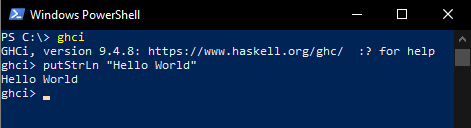
\includegraphics[width=1\linewidth]{Figures/Anhang/ghci}
    \caption{Verwendung von GHCi in der Windows PowerShell}
\end{figure}

Um Haskell Syntax und generelle Prinzipien zu lernen, wurden zunächst die ersten Aufgaben der CIS 194 Hausaufgaben bearbeitet.

%\end{FlushLeft}
%%%%%%%%%%%%%%%%%%%%%%%%%%%%%%%%%%%%%%%%%%%%%%%%%%%%%%%%%%%%%
%APPENDICES
%%%%%%%%%%%%%%%%%%%%%%%%%%%%%%%%%%%%%%%%%%%%%%%%%%%%%%%%%%%%%
%\appendix
%\renewcommand*{\thesection}{\Alph{section}}\textbf{}
% APPENDIX A
%\input{Appendices/Appendix_1.tex}
%%%%%%%%%%%%%%%%%%%%%%%%%%%%%%%%%%%%%%%%%%%%%%%%%%%%%%%%%%%%%
%BIBLIOGRAPHY
%%%%%%%%%%%%%%%%%%%%%%%%%%%%%%%%%%%%%%%%%%%%%%%%%%%%%%%%%%%%%
\newpage
\renewcommand*{\thesection}{}\textbf{}
\bibliographystyle{apacite}
\bibliography{Bibliography.bib}
\end{document} 
